\section{Application}

To empirically validate the feasibility of our proposed methodology, we developed a prototype application. This application contains it's frontend and backend. The backend  implements the generators and other services and provides them via an API. Users can use our frontend via web application that communicates with the backend. The web application contains a text area for inserting a domain description and a modeling canvas where the user creates the domain model using classical manual modeling features and the suggestion features highlighted by the \textit{magic wand} icon. \\

TODO: Brief chapter description \\

\subsection{Assistant services}

Our LLM based assistant provides the following services:
\begin{enumerate}
\item domain elements suggestion
\item highlighting already modeled elements
\item domain model summary
\end{enumerate}

\subsection{Domain elements suggestion}

When a domain description is provided the assistant generates suggestions solely based on the provided text. Otherwise, the assistant generates most relevant suggestions solely based on it's trained parameters.

Our assistant is able to suggest classes. For a selected class the assistant provides functionality to suggest it's attributes and associations. And for a selected source class and a selected target class the assistant is able to suggest their associations. Figure \ref{fig:assistant-features} demonstrates these features.

\begin{figure}[!h]
    \centering
    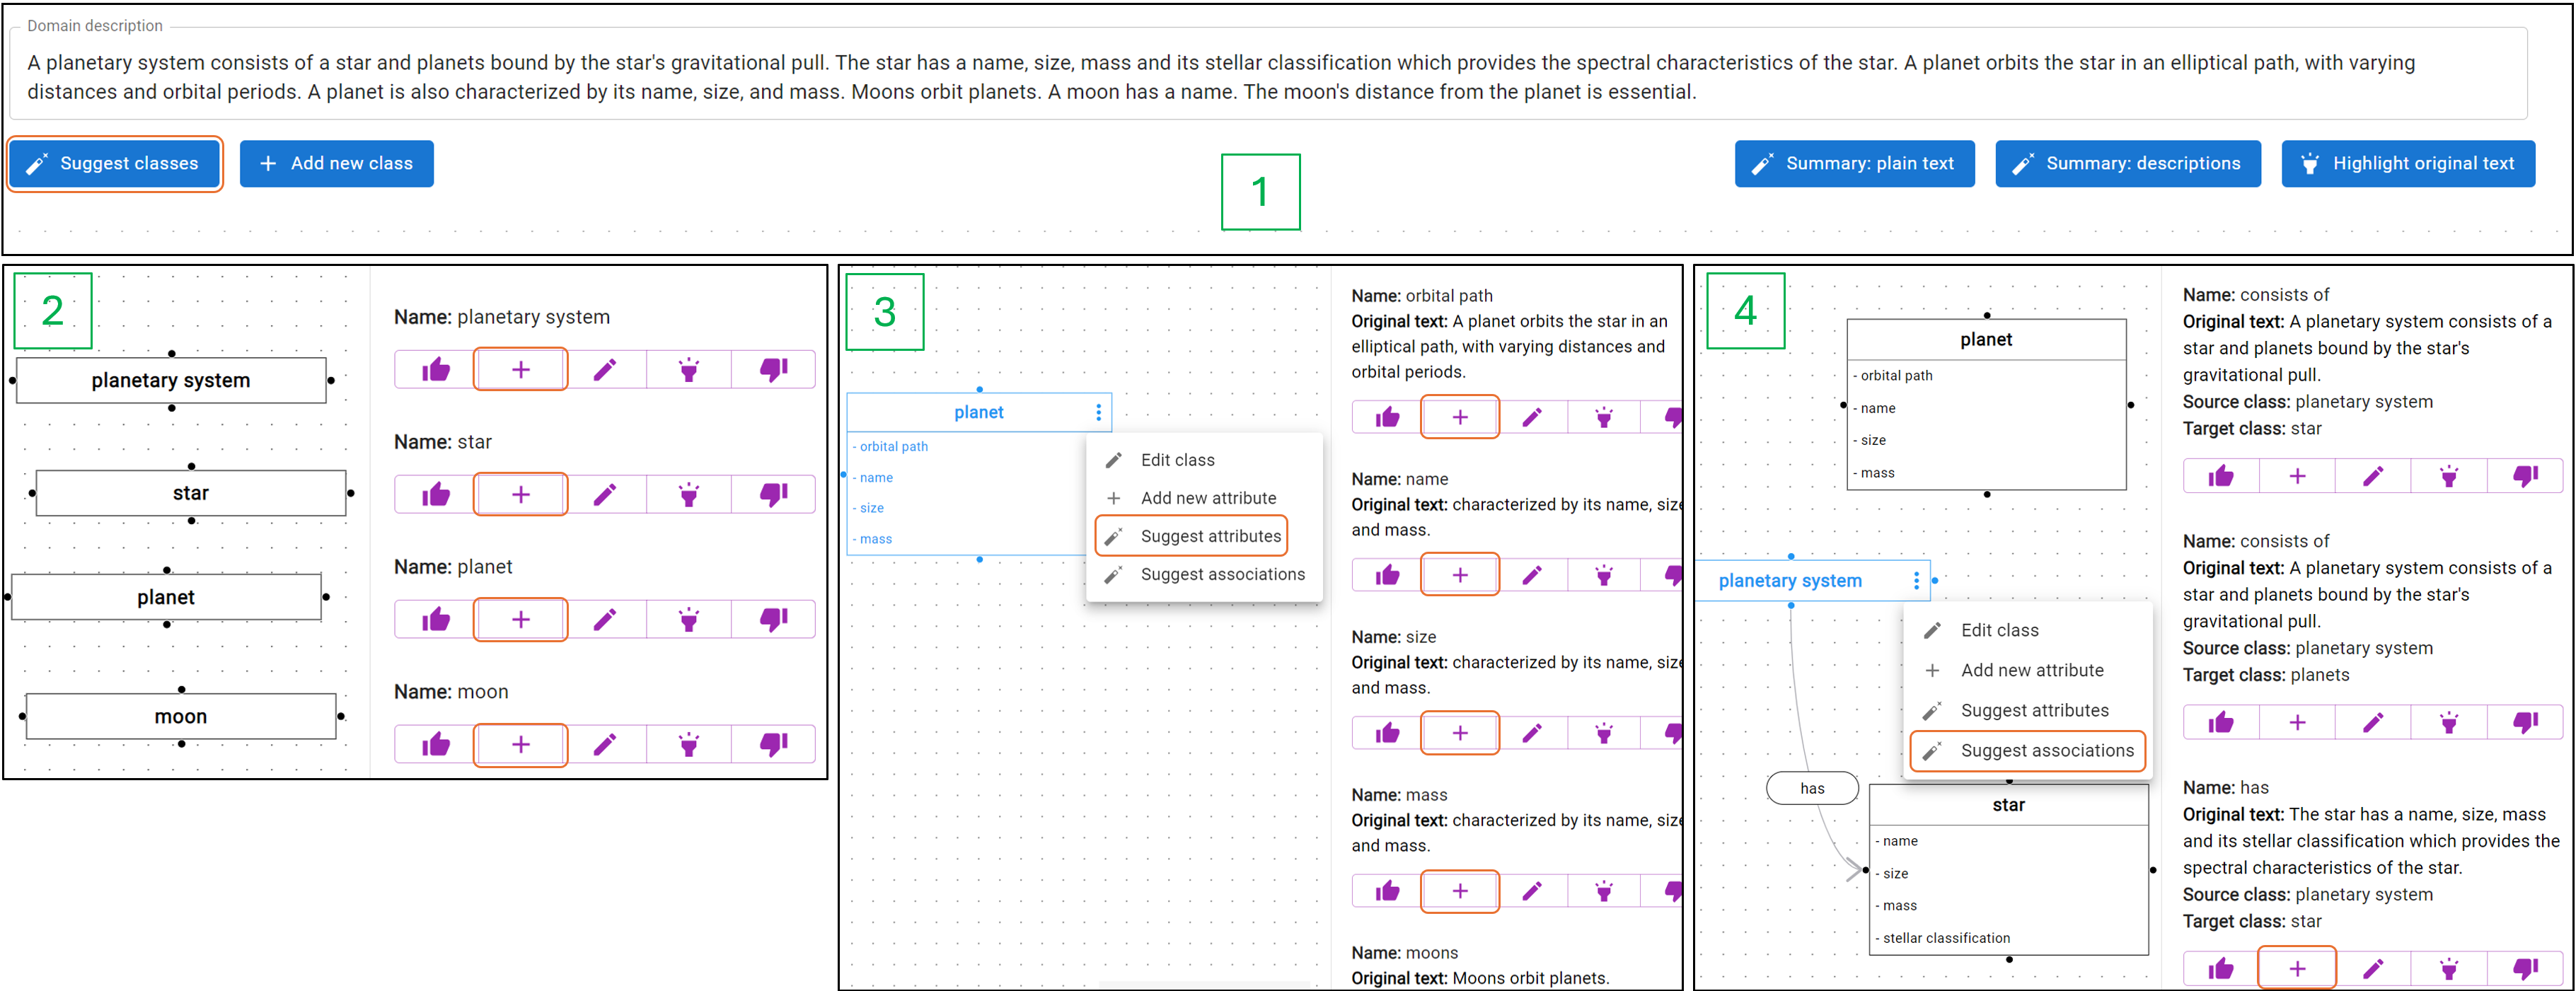
\includegraphics[scale=0.22]{img/assistant-features.png}
    \caption{\centering Screenshots of the main functionalities of the prototype application}
    \label{fig:assistant-features}
\end{figure}

Screenshot 1 shows the text area for the domain description and action buttons. The highlighted button \textit{Suggest classes} calls the $gen_c$ operator with the inserted domain description. Screenshot 2 shows the list of suggested classes. The user can use the highlighted ``+'' buttons to insert suggested classes into the modeling canvas. The other buttons are used for \textit{liking} and \textit{disliking} the corresponding suggestion, is editing before inserting t he suggested class into the canvas, and highlighting the suggestion in the original domain description. For the selected class, the user can ask for attribute and association suggestions, i.e. $gen_a$ and $gen_r$ operators for the class and the domain description. Screenshot 3 shows the attribute suggestions. Screenshot 4 shows the association suggestions. For the suggested attributes and association, the tool also shows the original text returned by the operators $gen_a$ and $gen_r$.


\subsubsection{Context highlighting}

As mentioned in the section (TODO: add section reference), for each suggested attribute and association we highlight it's context in the domain description. Additionally, for each class we highlight it's name.

This requires being able to match the LLM generated text with the domain description. The matching is easy as long as the generated text syntactically exactly matches some part of the domain description. %However, in some cases it makes sense to generate text that is not continuous in the domain description. For example: \\

%\noindent{\textit{Students have a name and address.}} \\

%\noindent{In this case the original text for the attribute ``address'' can look like this:} \\

%\noindent{\textit{Students have $\ldots$ address.}} \\

However, we encountered some common issues with this approach. For example, sometimes the LLM changes some letter when generating the text. For instance, when domain description contains the word ``motorized'' with the ``z'' letter the LLM can generate the word ``motorised'' with the ``s'' letter instead.

To mitigate this issue we implemented a simple recovery strategy. When the generated text and the domain description cannot be directly matched we find their longest common substring and we split the generated text into the longest common substring and the remaining parts. Subsequently, we try to match these parts without the letter that was in the middle of these parts.


\subsubsection{Single field suggestion}

For the best possible LLM output quality and response time when generating suggestions we try to simplify the prompts as much as possible. This for example means that the generated attributes suggestions does not contain their description or data type. For generating these additional fields our assistant can be used. \\

TODO: Vyjmenovat ty generátory, které tady používáme. \\

TODO: zmínit nastavení formátu pro jména až to budu mít naimplementované \\


\subsubsection{Attributes and associations conversion}

Attributes can be usually modeled as an associations and vice versa. For example, ``address'' can be an attribute of a class ``person'' but it also can be an association in between the classes ``person'' and ``address''. Therefore, for each attribute suggestion we provide functionality to convert them to an association and vice versa. We convert an attribute into an association by putting the attribute name into the association target class and we put the attribute name into the association name. As the copied name does not have to fit the LLM assistant can be used to generate a new name. The opposite conversion works the same but in reverse.


\subsubsection{Duplicate domain elements}
\label{duplicate_domain_elements}
The generated domain element suggestion is not shown to the user if he already modeled the corresponding element. We remove these suggestions on the backend after the LLM generates the output so we do not have to provide the user's domain model in the prompts for generating classes, attributes and associations.

The domain element suggestion is removed if it's name syntactically matches the name of the user's corresponding modeled element. This approach has the following limitations.

First limitation is that if two domain elements have the same name but a different semantics then a relevant domain element is removed. For example, the class ``car'' can have attribute ``year'' referring to the year of the car manufacturing and the same attribute referring to the year of technical inspection. In our experience, this issue is very rare as the LLM usually generates suggestions with explicit names so in this case the first mentioned attribute would probably be name ``year of manufacturing'' and the second attribute would probably be named ``year of technical inspection''. However, if more of these issues occur, removal of duplicate domain elements can be disabled.

Second limitation is that semantically same domain elements with a different name are not removed. Possible solutions are to either use a LLM or some BERT based model as in retrieval-augmented generation for semantic comparison. However, both have significant disadvantages. Solving the mentioned problem with a LLM in a single prompt approach complicates the prompt wording and can reduce the output quality. Using LLM in an iterative prompt approach can significantly increase the delay between the user's request and the suggestions displaying as the LLM has to process more than one prompt which can take many seconds. When using some BERT based model as mentioned in the section (TODO: section reference), one of the challenging tasks is to set the decision boundary between accepting and rejecting the corresponding element. For example attributes ``first name'' and ``last name'' are very close in terms of vector space distance however, they represent a two semantically distinct different attributes. This fact would force us to set very strict decision boundary that would reject almost any two syntactically different words which is in result almost identical to our naive approach.


\subsection{Highlighting already modeled elements}

We extend the mentioned highlighting of elements in the domain description by highlighting all the user's modeled elements in the domain description. \\

TODO: na jaké hlavní problémy jsem narazil a proč některé zvýrazněné prvky v popisu domény ve skutečnosti nemusí být namodelovány a naopak viz poznámky \\


\subsection{Summary of domain model}

For a selected part of the user's conceptual model the assistant is able to generate a summary for each class, attribute and association. We implemented two summary variations: in a plain text and in form of bullet points.

In both variations the corresponding prompt does not contain the user's domain description because we found out that our used LLM does not stick to the selected conceptual model when it gets both the user's conceptual model and the domain description as the input.

The plain text summary generates a paragraph describing the user's selected domain model. We let the user to set the style of this summary. The available styles are ``analytical'', ``educational'' and ``funny story''. When a style is selected the prompt for plain text summary is edited so it instructs the LLM to generate the output in the selected style.

The summary in form of bullet points for each element generates a description. In the future by adding options to accept, reject or regenerated each description this could be used to help the user to create a description for each of his modeled element for a better domain model documentation.


\subsection{LLM parameters}

For each task we set the temperature to $0$ as we usually want the LLM to only generate the most probable output as discussed in the section \ref{temperature}.

Other parameters are set to their default values which are defined in the OpenAI API\footnote{\url{https://platform.openai.com/docs/api-reference/introduction}}.


\subsection{LLM output parsing}

TODO: zmínit hlavní věci, které se dějí při parsování výstupu + odkázat se na to, že odstraňování duplicitních elementů jsme již pokryli v předchozí subsekci \\


\subsection{Saving user data}

For each generated suggestion the user can optionally click on the like button or the dislike dislike button. The corresponding evaluated suggestion is sent to the backend and saved there with all the parameters that were used to generate this suggestion. To remember these parameters, the frontend remembers for each suggestion the parameters that were used for generation.

We use these user's reactions for two main reasons. First reason is that we can use these data as a feedback. For example, we can automatically detect if some set of parameters repeatedly ended up with too many negative reactions. After that we can analyse the issue and fix it. Second reason is that we can use these data to fine-tuning some LLM to further improve the quality for our specific tasks.

The downside of our approach is that it does not collect many user data. One possible solution is to save each user action such as saving each suggestion that the user added into his domain model. However, this approach has a lot of disadvantages due to it's complexity. For example, if the user adds some suggestion and then later on removes it we need to save this removal action too as it can mean that the original suggestion turned out to be unwanted. This means that the saved data would need to be post-processed to remove these pairs of data. Similar issue arise when user adds some suggestion but then later on edits it. Because of this complexity we decided to use the explicit reactions buttons.


\subsection{Work-flow}

Figure \ref{fig:work-flow} shows the basic flow of generating suggestions on the backend.

\begin{figure}[!h]
    \centering
    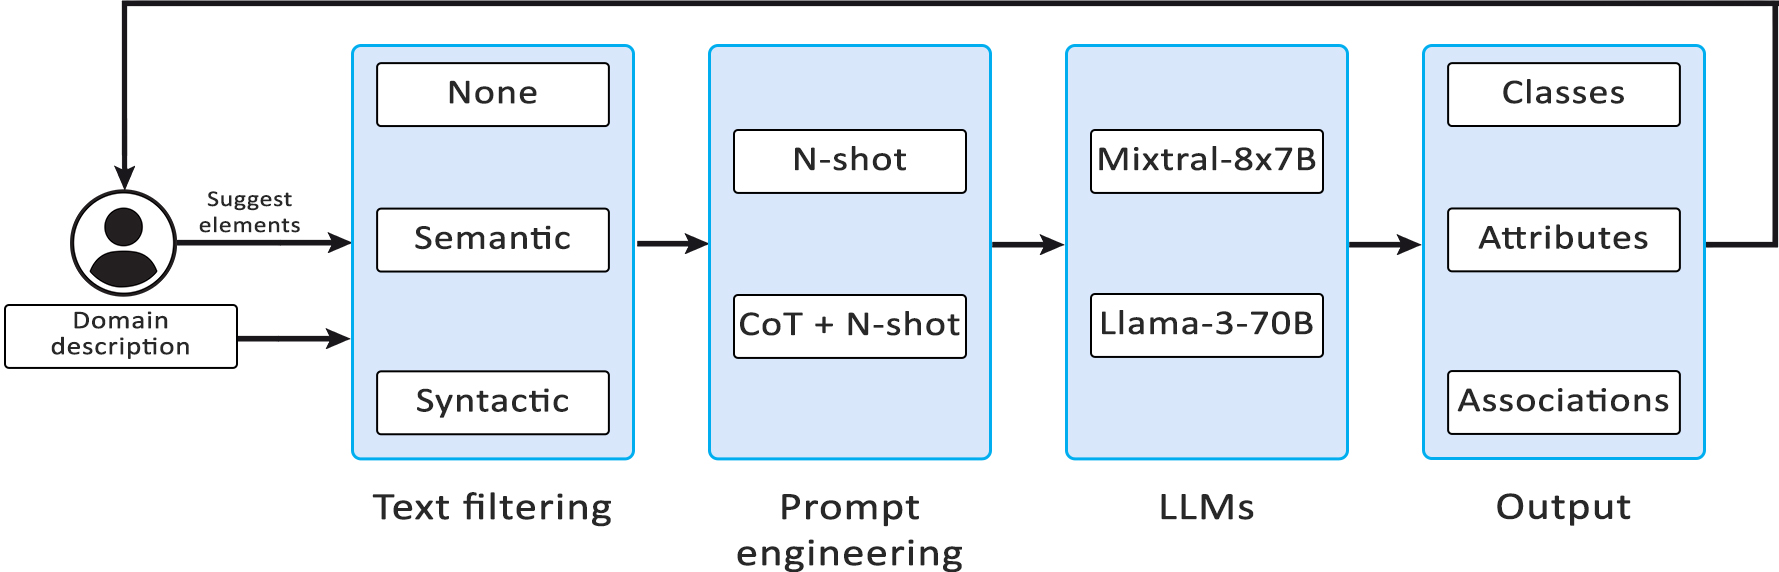
\includegraphics[scale=0.23]{img/work-flow.jpg}
    \caption{\centering Schema of the flow of processing the textual domain description}
    \label{fig:work-flow}
\end{figure}

The modeling process typically starts by providing the domain description. Then the domain model is step by step created by using suggestions from the assistant. Suggestions of attributes and associations are filtered by the selected retrieval-augmentation generation method. Then the prompt engineering techniques are applied and the final prompt is constructed and sent to LLM. Finally, the output from the LLM is parsed and the suggested model elements are sent back to the frontend.